% Copyright (c) 2022 by Lars Spreng
% This work is licensed under the Creative Commons Attribution 4.0 International License. 
% To view a copy of this license, visit http://creativecommons.org/licenses/by/4.0/ or send a letter to Creative Commons, PO Box 1866, Mountain View, CA 94042, USA.

%~~~~~~~~~~~~~~~~~~~~~~~~~~~~~~~~~~~~~~~~~~~~~~~~~~~~~~~~~~~~~~~~~~~~~~~~~~~~~~
% You can add your packages and commands to the loadslides.tex file. 
% The files in the folder "styles" can be modified to change the layout and design of your slides.
% I have included examples on how to use the template below. 
% Some of these examples are taken from the Metropolis template.
%~~~~~~~~~~~~~~~~~~~~~~~~~~~~~~~~~~~~~~~~~~~~~~~~~~~~~~~~~~~~~~~~~~~~~~~~~~~~~~


\documentclass[
11pt,notheorems,hyperref={pdfauthor=whatever}
]{beamer}

\input{loadslides.tex} % Loads packages and some defined commands

\title[
% Text entered here will appear in the bottom middle
]{Ensemble learning}

\subtitle{How to use multiple times the same data}

\author[
% Text entered here will appear in the bottom left corner
]{
    Michele Vincenzo Branca, Leonardo De Pietro
}

\institute{
    Collegio Carlo Alberto, \\
    University of Turin}
\date{April 29, 2026}

% packages
\usepackage{amsmath}

\begin{document}

% Generate title page
{
\setbeamertemplate{footline}{} 
\begin{frame}
  \titlepage
\end{frame}
}
\addtocounter{framenumber}{-1}

\begin{frame}{Index of the presentation}
    % This stacks the sections from all three parts into one unified list
    \tableofcontents[part=1, hideallsubsections]
    \tableofcontents[part=2, hideallsubsections]
    \tableofcontents[part=3, hideallsubsections]
\end{frame}

\makepart{What is Ensemble Learning?}
\justifying
\section{What is Ensemble Learning?}
\subsection{An overview}
\begin{frame}
    Given a \emphasize{\textbf{supervised learning algorithm}} \(\mathcal{A}(\mathcal{D})\,:\,\mathcal{X}\to\mathcal{Y}\), can we run it more than once on datasets constructed from the original one \(\mathcal{D}\) and then combine the results to get an overall better predictor? Kind of.
    
    First of all, what kind of combinations are we (typically) talking about?
    \begin{itemize}
        \item linear ones!
    \end{itemize}
    How do we do it for various algorithms?
    \begin{itemize}
        \item \alert{\textbf{local averaging methods}}: combine the predicted labels from estimators learned on different datasets;
        \item \alert{\textbf{regression}}: linearly combine the predictions;
        \item \alert{\textbf{classification}}: weighted majority vote or linear combination of real-valued predictions when convex surrogates are used.
    \end{itemize}
    What's the impact?
    \begin{itemize}
    \item for \example{\textbf{linear models}} this method does not add new functions;
    \item for \example{\textbf{non-linear models}} this method can add new functions. 
\end{itemize}
\end{frame}

\subsection{How to construct the datasets?}
\begin{frame}
    Suppose that \(\mathcal{D}\) is the original dataset. 

    We construct new datasets by assigning different weights to the data points. According to the weights' nature, they have different interpretations:
    \begin{itemize}
        \item \alert{\textbf{integer-valued weights}}: the new dataset is obtained by including the points the number of times specified by the weights;
        \item \alert{\textbf{(non-negative) real-valued weights}}: implemented by sampling points proportionally to their weights during training, effectively treating the normalized weight as a sampling probability (e.g., in \example{\textbf{SGD}});
        \item \alert{\textbf{arbitrary weights}}: modern techniques based on empirical risk minimization directly accomodate arbitrary weights. 
    \end{itemize}
    We will focus on \example{\textbf{bagging/averaging}} techniques:
    \begin{itemize}
        \item datasets constructed in parallel with \alert{\textbf{random weights}} (typically uniform) or - which yields similar results - using \alert{\textbf{random projections}}.
    \end{itemize}
\end{frame}

\subsection{A spoiler: what are the computational and statistical benefits?}
\begin{frame}
    It really depends on the original predictors:
    \begin{itemize}
        \item \alert{\textbf{local averaging methods}}: ensemble learning will typically \example{\textbf{reduce the variance}} of the predictor and parallalelization \example{\textbf{reduces the computational complexity}};
        \item \alert{\textbf{empirical risk minimization with nonlinear models}}: linear combinations \example{\textbf{increase the set of models}} from \(\varphi(\cdot,\,w)\) to \(\int\limits_{\mathcal{W}}\varphi(x,\,w)\,\mathrm{d}\nu(w)\), where \(\nu\) is a signed measure on \(\mathcal{W}\). Furthermore, \example{\textbf{variance and computational cost are decreased}};
        \item \alert{\textbf{empirical risk minimization with linear models}}: a linear combination of linear models will still be a linear models, thus not increasing the set of models. However, there are usually great \example{\textbf{computational benefits}}.
    \end{itemize} 
\end{frame}

\makepart{Averaging/Bagging}
\justifying
\section{Averaging}
\subsection{The framework}
\begin{frame}
    We will consider \alert{\textbf{regression with square loss}} where we have an explicit \example{\textbf{variance/bias}} decomposition.
    \begin{itemize}
        \item most results extend to other situations using convex surrogates.
    \end{itemize}
\end{frame}

\subsection{Averaging: the idealized setting}
\begin{frame}
    Suppose we have \(m\) indipendent datasets of size \(n\), all coming from an i.i.d. sample having the same distribution \(p(x,\,y)\) on \(\mathcal{X}\times\mathcal{Y}\). From each of them, we get an estimator:
    \[
        \hat{f}^{(j)},\quad j=1,\dots,\,m,
    \]
    and the new predictor is:
    \[
        \hat{f}^{\text{bag}}(x) = \frac{1}{m} \sum_{j=1}^m \hat{f}^{(j)}(x).
    \]
    Denote:
    \begin{itemize}
        \item \(\text{bias}^{(j)}(x)=\mathbb{E}\left[\hat{f}^{(j)}(x)\right]-f_*(x)\);
        \item \(\text{var}^{(j)}(x)=\text{var}\left[\hat{f}^{(j)}(x)\right]\);
    \end{itemize}
    where we assume that \(x\) is fixed, thus the expectations are taken with respect to the data only. Note that:
    \begin{itemize}
        \item \(\text{bias}^{\text{bag}}(x)=\text{bias}^{(j)}(x)\) for any \(i=1,\dots,\,m\);
        \item \(\text{var}^{\text{bag}}(x)=\text{bias}^{(j)}(x)\) for any \(i=1,\dots,\,m\);
    \end{itemize}
    because of i.i.d. assumption. 
\end{frame}

\subsection{Example: \(k\)-nearest neighbor regression}
\begin{frame}
    Take \(\mathcal{X}\subset\mathbb{R}^d\). In this case we have that the expected excess risk is upper bounded in this way\footnote{See Proposition 6.2, p. 170 \textit{Learning Theory from First Principles}, by \textit{Francis Bach}.}:
    \[
        \int_{\mathcal{X}}\mathbb{E}\left[(\hat{f}(x)-f_\star(x))^2\right]\mathrm{d}p(x)\leq\underbrace{\frac{\sigma^2}{k}}_{\text{variance upper bound}}+\underbrace{8B^2\text{diam}(\mathcal{X})^2\left(\frac{2k}{n}\right)^{2/d}}_{\text{bias upper bound}},
    \]
    where:
    \begin{itemize}
        \item \(\mathcal{X}\) is the \alert{\textbf{input feature space}} and \(\mathcal{Y}\) is the \alert{\textbf{output space}};
        \item \(f_\star\in\argmin\limits_{y\in\mathcal{Y}}\mathbb{E}\left[\ell(y,\,z)\mid x\right]\) is the \alert{\textbf{Bayes predictor}};
        \item \(\hat{f}(x)\) is the \alert{\textbf{prediction}} made by the \alert{\textbf{\(k\)-nearest neighbor estimator}} at a specific \alert{\textbf{evaluation point}} \(x\);
        \item \(p(x)\) is the \alert{\textbf{marginal probability distribution}} of the input features;
        \item \(\sigma^2\) is the \alert{\textbf{irreducible error}} \(\text{var}(y \mid x)\);
        \item \(B\) is the \alert{\textbf{Lipschitz constant}} of the Bayes predictor \(f_\star(x)\);
        \item \(\text{diam}(\mathcal{X})\) is the \alert{\textbf{maximum possible distance}} between any two points in the space.
    \end{itemize}   
\end{frame}
\begin{frame}    
    Thus, \alert{\textbf{averaging}} over \(m\) replications, we get that the \example{\textbf{excess risk}} is upper bounded by:
    \[
        \int_{\mathcal{X}}\mathbb{E}\left[(\hat{f}(x)-f_\star(x))^2\right]\mathrm{d}p(x)\leq\frac{\sigma^2}{\textcolor{red}{m}k}+8B^2\text{diam}(\mathcal{X})^2\left(\frac{2k}{n}\right)^{2/d},
    \]
    and optimizing over \(k\) yields: \(k\propto \frac{1}{m^{d/(2+d)}}\cdot n^{2/(2+d)}\). The overall excess risk ends up being proportional to \(1/(mn)^{2/(2+d)}\), which coincides with the rate for a dataset with \(N=nm\) observations.
    
    Clearly we have a limit concerning the number  of datasets we can construct: we need \(k>1\), thus substituting in this condition the optimal \(k\) (which is a function of \(m\) and \(n\)) we see that \(m\) cannnot grow larger than \(n^{2/d}\).
\end{frame}

\subsection{Example: Ridge regression (misspecified model)}
\begin{frame}
    In this case we have that the expected excess risk is upper bounded in this way\footnote{See Proposition 7.8, p. 216 \textit{Learning Theory from First Principles}, by \textit{Francis Bach}.}:
    \[
        \int_{\mathcal{X}}\mathbb{E}\left[(\hat{f}(x)-f_\star(x))^2\right]\mathrm{d}p(x)\leq\underbrace{\frac{\sigma^2}{n}\left(1+\frac{R^2}{\lambda n}\right)\text{tr}\left(\left(\Sigma+\lambda I\right)^{-1}\Sigma\right)}_{\text{variance upper bound}}+\underbrace{\left(1+\frac{R^2}{\lambda n}\right)^2\inf\limits_{f\in\mathcal{H}}\{\mid\mid f-f_\star\mid\mid^2_{L_2(p)}+\lambda\mid\mid f\mid\mid_{\mathcal{H}}^2\}}_{\text{bias upper bound}},
    \]
    where:
    \begin{itemize}
        \item \(\mathcal{X}\), \(f_\star\), \(\hat{f}\), \(p(x)\), \(\sigma^2\) represent the same things as before,
        \item \(\lambda\) is the \alert{\textbf{regularization parameter}}, which controls the trade-off between fitting the training data and keeping the model weights small;
        \item \(\Sigma\) is the \alert{\textbf{covariance matrix}} of the features in the feature space;
        \item \(R^2\) is a \alert{\textbf{bounding constant}} related to the norm of the features;
        \item \(\mathcal{H}\) is the \alert{\textbf{Reproducing Kernel Hilbert Space (RKHS)}} (or hypothesis space) where the candidate functions \(f\) live;
        \item \(\text{tr}\left(\left(\Sigma+\lambda I\right)^{-1}\Sigma\right)\) are the \alert{\textbf{degrees of freedom}} associated to the covariance operator \(\Sigma\).
    \end{itemize}  
\end{frame}

\begin{frame}    
    For the \example{\textbf{bias term}}, assuming:
    \begin{itemize}
        \item \(\mathcal{X}=\mathbb{R}^d\);
        \item that the target function belongs to a Sobolev Kernel of order \(t>0\);
        \item that \(\mathcal{H}\) is a Sobolev space of order \(s>d/2\); 
    \end{itemize}
    one gets that the bias term is of order \(\left(1+\frac{R^2}{\lambda n}\right)^2\lambda^{t/s}\). 
    
    For the \example{\textbf{variance term}}, assuming:
    \begin{itemize}
        \item that the eigenvalues \((\lambda_m)\) of the covariance matrix \(\Sigma\) satisfy \(\lambda_m\leq C(m+1)^{\alpha}\), \(\alpha>1\);
    \end{itemize} 
    then \(\text{tr}\left(\left(\Sigma+\lambda I\right)^{-1}\Sigma\right)\leq O(\lambda^{1/\alpha})\). With our \(\mathcal{X}\), \(\alpha=2s/d\), thus the variance is proportional to \(\frac{1}{n}\lambda^{-d/(2s)}\)\footnote{See section 7.6.6, p. 217 \textit{Learning Theory from First Principles}, by \textit{Francis Bach}.}.

    \alert{\textbf{Averaging}} over \(m\) replications, we get that the \example{\textbf{excess risk}} is proportional to \(\frac{\sigma^2}{nm}\lambda{-1/\alpha}+\lambda^{t/s}\), and again the estimator behaves like having \(N=nm\) observations.
\end{frame}

\section{Bagging}
\subsection{The framework}
\begin{frame}
    We will consider again \alert{\textbf{regression with square loss}} where we have an explicit \example{\textbf{variance/bias}} decomposition.
    \begin{itemize}
        \item most results extend to other situations using convex surrogates.
    \end{itemize}
    We suppose we have datasets \(\mathcal{D}^{(b)}\), \(b=1,\dots,m\). Fixing \(b\), each of them obtained with \alert{\textbf{random weights}} \(v_i^{(b)}\in\mathbb{R}_+\,i=1,\dots,n\). Recall that in the case of natural numbers that sum up to \(n\) we are in the setting of bootstrapping.

    We study \(m=\infty\), even though in pratice approximately asymptotic performances are achieved for moderate \(m\)'s.

    For linear estimators (e.g. \example{\textbf{kernel ridge regression}} or \example{\textbf{local averaging}}) this procedure yields another linear estimator with a \example{\textbf{lower variance}} and an unchanged \example{\textbf{bias}}
    \begin{itemize}
        \item in this sense, bagging can be seen as another way of \alert{\textbf{regularizing}}.
    \end{itemize} 
    This means that there's no strong statistical gain, but rather a computational one.

\end{frame}


\subsection{Example: one-nearest neighbor regression}
\begin{frame}
    Denote as \((x_{(i)}(x),\,y_{(i)}(x))\) the \(i\)-th closest neighbor of \(x\) from the dataset \(x_1,\dots,x_n\), we can write the \alert{\textbf{bagged}} estimate as:
    \[
    \hat{f}(x)=\sum\limits_{i=1}^nV_iy_{(i)}(x).
    \]
    The weights \(V_i\) sum to \(1\) (interpret \(V_i\) as the probability that the \(i\)-th nearest neighbor of \(x\) is also the \(i\)-th nearest in a uniform subsample of a certain size \(s\), where we assume \(s\geq2\)) and do not depend on \(x\).

    \begin{itemize}
        \item For the \alert{\textbf{viarence}} term we have \(\text{var}(\hat{f}(x)) = \sigma^2 \sum_{i=1}^n V_i^2\) where we can bound by a combinatorial argument \(\sum^n V_i^2\) by \(\sum\limits_{i=1}^nV_i^2\leq\frac{s}{n}\frac{1}{(1+1/n-s/n)^2}\).
        \item For the \alert{\textbf{bias}} term, using \(y_{(i)}=f_\star(x_{(i)})+\varepsilon_i\), assuming \(f_\star\) to be \(B\)-Lipschitz continuous we can bound \(\mathbb{E}[\hat{f}(x)] - f_\star(x)\) by \(4B^2\text{diam}(\mathcal{X})^2\frac{1}{s^{2/d}}\)
    \end{itemize}

    Thus, the overall \alert{\textbf{excess risk}} is bounded by:
    \[
        4B^2\text{diam}(\mathcal{X})^2\frac{1}{s^{2/d}}+\frac{s}{n}\frac{1}{(1+1/n-s/n)^2}.
    \]
    This can be balanced by choosing \(s^{1+2/d}\propto n\), leading to performance as the \(k\)-nearest neighbor for a well chosen \(k\), but with a bagged estimate.
\end{frame}

\begin{frame}{}{Example: one-nearest neighbor regression -- picture}
    \centering
    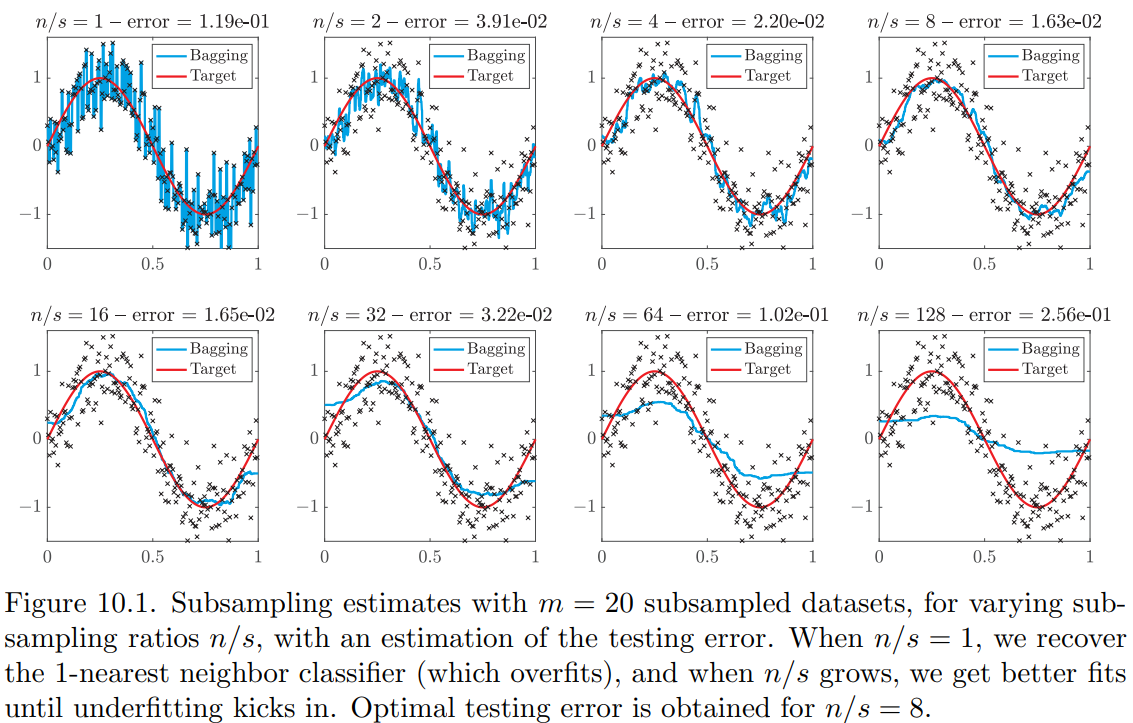
\includegraphics[width=0.8\textwidth]{img.png}
\end{frame}

\makepart{Random projections and averaging}
\justifying
\section{The Two Paradigms}
\subsection{Overview of Data Compression}
\begin{frame}
    In the previous section, we reweighted observation to be able to re-run the original algorithm, this can also be done through random projection.
    We consider two settings:
    \begin{itemize}
        \item \alert{\textbf{Sketching (\(S \in \mathbb{R}^{s \times n}\))}}: shrinking the datapoints (rows). We compress \(n\) observations into \(s\) new observations (\(n > s > d\)) by replacing \(\min_{\theta \in \mathbb{R}^d}\|y - \Phi\theta \|^2_2 \) by \(\min_{\theta \in \mathbb{R}^d}\|Sy - S\Phi\theta \|^2_2 \) where \(S\) is an i.i.d Gaussian matrix.
        \item \alert{\textbf{Random Projection (\(S \in \mathbb{R}^{d \times s}\))}}: shrinking the features (columns). We constrain our search space to an \(s\)-dimensional subspace (\(d > n > s\)) by replacing \(\min_{\theta \in \mathbb{R}^d}\|y - \Phi\theta \|^2_2 \) by \(\min_{\eta \in \mathbb{R}^s}\|y - \Phi S \eta \|^2_2 \).
    \end{itemize}
    What are the primary benefits?
    \begin{itemize}
    \item \example{\textbf{Sketching}} provides computational and storage benefits (reducing \(\mathbb{R}^{n \times d}\) to \(\mathbb{R}^{s \times d}\)).
    \item \example{\textbf{Random Projections}} provide both a reduction in computation time and inherent \example{\textbf{regularization}} in high-dimensional setups.
\end{itemize}
\end{frame}

\section{Gaussian Sketching}
\subsection{The Framework}
\begin{frame}
    Following the ordinary least-squares framework, we consider a design matrix \(\Phi \in \mathbb{R}^{n \times d}\) with full column rank \(d\) (thus \(n \ge d\)). 
    
    We generate \(m\) replications using Gaussian sketching matrices \(S^{(j)} \in \mathbb{R}^{s \times n}\). The \alert{\textbf{sketched closed-form estimator}} is:
    \[
        \hat{\theta}^{(j)} = (\Phi^\top(S^{(j)})^\top S^{(j)}\Phi)^{-1}\Phi^\top(S^{(j)})^\top S^{(j)}y
    \]
    and our final ensemble predictor is:
    \[
        \hat{\theta} = \frac{1}{m} \sum_{j=1}^m \hat{\theta}^{(j)}
    \]
    
    Computing expectation with respect to the random sketching we get \(\mathbb{E}_{S^{(j)}}[\Phi\hat{\theta}^{(j)}] = \Phi\hat{\theta}_{\text{OLS}}\), so Gaussian sketching provides an \alert{\textbf{unbiased}} estimator of the \alert{\textbf{true OLS prediction}}, while the variance term is \(\mathbb{E}_{\varepsilon, S^{(j)}}\left[ \big\|\Phi\hat{\theta}^{(j)} - \mathbb{E}_{S^{(j)}}\Phi\hat{\theta}^{(j)}\big\|_2^2 \right] = \sigma^2 \frac{d(n-d)}{s-d-1}\)
\end{frame}


\subsection{Expected Generalization Error}
\begin{frame}
    Combining the Bias and Variance terms for our ensemble of \(m\) independent sketches, the expected generalization error is:
    \[
        \frac{1}{n} \mathbb{E}_{\varepsilon, S} \Bigg[ \bigg\| \frac{1}{m} \sum_{j=1}^m \Phi\hat{\theta}^{(j)} - \Phi\theta_* \bigg\|_2^2 \Bigg] = \frac{\sigma^2 d}{n} + \textcolor{red}{\frac{\sigma^2 d}{n}\left(\frac{1}{m}\frac{n-d}{s-d-1}\right)}
    \]
    where:
    \begin{itemize}
        \item \(\frac{\sigma^2 d}{n}\) is the \alert{\textbf{standard OLS error}} baseline;
        \item the \textcolor{red}{red term} is the \alert{\textbf{algorithmic sketching penalty}};
    \end{itemize}

    What does this bound tell us about the trade-offs?
    \begin{itemize}
        \item as \example{\(m \to \infty\)}: the penalty vanishes. Averaging infinitely many sketches perfectly reconstructs the original OLS estimator.
        \item to \example{\textbf{match OLS performance}} (up to a factor of 2), we need the penalty term to equal the base error. This requires \(m \sim \frac{n}{s}\) replications.
    \end{itemize}
    \vspace{0.25cm}
    \textbf{Conclusion:} Just like bagging, there is \emphasize{\textbf{no statistical gain}} over OLS. The benefit is purely computational. We can process \(m\) tiny datasets of size \(s \times d\) in parallel instead of one massive dataset of size \(n \times d\).

\end{frame}

\section{Random Projections}
\subsection{The High-Dimensional Setting}
\begin{frame}
    We now put ourselfs in an high-dimension set-up: assume \(d > n\).
    \begin{itemize}
        \item \example{Standard OLS} is \alert{ill-posed} because \(\Phi^\top\Phi\) is not invertible.
    \end{itemize}

    A possible solution is:
    \begin{itemize}
        \item For each \(j = 1,\dots,m\), use \alert{sketching} matrix \(S^{(j)} \in \mathbb{R}^{d \times s}\) (\(s \le n\)), we assume \(\text{rank}(S^{(j)}) = s\) a.s. .
        \item We \alert{restrict the searching} space considering \(\hat{\theta}^{(j)} = S^{(j)}\hat{\eta}^{(j)}\) where \(\hat{\eta}^{(j)}\) minimizes \(\min_{\eta \in \mathbb{R}^s} \|y - \Phi S^{(j)}\eta\|_2^2\)
        \item The denoised resposnse vector is \(\hat{y}^{(j)} = \Pi^{(j)} y\), where \(\Pi^{(j)}\) is an \alert{orthogonal projection matrix} onto an \(s\)-dimensional vector space, such that, denoting its expectation \(\Delta = \mathbb{E}[\Pi^{(j)}]\), \(\text{tr}(\Delta) = s\).
    \end{itemize}
    
\end{frame}

\subsection{Expected Excess Risk Bound}
\begin{frame}
    A first bound of the expected generalization error is 
    \[\frac{1}{n} \mathbb{E}_{\varepsilon, S} [ \| \frac{1}{m} \sum_{j=1}^m \hat{y}^{(j)} - \Phi\theta_* \|_2^2 ] \le \frac{\sigma^2 s}{n} + \frac{1}{n} \theta_*^\top \Phi^\top [I - \Delta] \Phi\theta_*.\]
    Now using the properties of the expectation of projection matrix to bound \(I - \Delta\) we get 
    \begin{equation}
        \frac{1}{n} \mathbb{E}_{\varepsilon, S} [ \| \frac{1}{m} \sum_{j=1}^m \hat{y}^{(j)} - \Phi\theta_* \|_2^2 ] \le  \frac{\sigma^2 s}{n} + \frac{1}{n} \theta_*^\top \Phi^\top H \footnote{\text{Where } \(H = \Big( I - \Phi \mathbb{E}_S \big[SS^\top\big] \big( \mathbb{E}_S \big[SS^\top \Phi^\top \Phi SS^\top\big] \big)^{-1} \mathbb{E}_S \big[SS^\top\big] \Phi^\top \Big)\)} \Phi\theta_*.
    \end{equation}
    Finally assuming the case of Gaussian random projections, the expected excess risk is bounded by:
    \[
        \underbrace{\frac{\sigma^2 s}{n}}_{\text{variance upper bound}} + \underbrace{\frac{2}{n}\text{tr}(\Phi^\top\Phi)\frac{\|\theta_*\|_2^2}{s+1}}_{\text{bias upper bound}}
    \]
    where:
    \begin{itemize}
        \item \(s\) acts as the \alert{\textbf{inverse regularization parameter}} (similar to \(1/\lambda\) in Ridge Regression)
    \end{itemize}
\end{frame}

\subsection{Exercise 10.4: Feature Subsampling}

\begin{frame}
    What if we replace the dense Gaussian matrix with a sparse one? 

    Consider a sketching matrix \(S \in \mathbb{R}^{d \times s}\), where each column is a \alert{\textbf{canonical basis vector}} \(e_i\). This is identical to randomly \example{\textbf{subsampling \(s\) features}} out of \(d\).

    Using the the bias bound from eq. (1) and using the moments of the Multinomial distribution we get an \example{\textbf{overall expected excess risk}}:
    \[
        \underbrace{\frac{\sigma^2 s}{n}}_{\text{variance}} + \underbrace{\frac{1}{n} \left( \frac{d}{s} \max_i(\|\phi_i\|_2^2) \|\theta_*\|_2^2 \right)}_{\text{bias upper bound}}
    \]

    \textbf{Conclusion:}
    \begin{itemize}
        \item The bias term scales as \(\frac{d}{s}\) instead of \(\frac{1}{s}\) (Gaussian case). You need \(s \propto d\) to achieve the same regularization.
        \item The bias penalty is now governed by the \alert{\textbf{maximum column norm}} \(\max_i(\|\phi_i\|_2^2)\) instead of the full trace \(\text{tr}(\Phi^\top\Phi)\).
        \item However, it provides better \alert{\textbf{computational performance}} since no dense \(\mathcal{O}(nd^2)\) matrix multiplications are required.
    \end{itemize}
\end{frame}


\section{Extensions: Kernel Methods}

\subsection{Infinite-Dimensional Models and RKHS}

\begin{frame}
    \textbf{Setup \& The Kernel Trick}
    \begin{itemize}
        \item \textbf{Data:} \(x \in \mathcal{X}\) (Input Space)
        \item \textbf{Feature Map:} \(\varphi: \mathcal{X} \rightarrow \mathcal{H}\), where \(\mathcal{H}\) is an infinite-dimensional \emphasize{\textbf{RKHS}}.
        \item \textbf{Kernel Function:} \(k(x, x') = \langle \varphi(x), \varphi(x') \rangle_{\mathcal{H}}\)
        \item We access \(\mathcal{H}\) exclusively through \(k(x, x')\), avoiding explicit computation of the infinite-dimensional \(\varphi(x)\).
    \end{itemize}
    
    \vspace{0.3cm}
    \textbf{Key RKHS Properties}
    \begin{itemize}
        \item \alert{\textbf{Reproducing Property}}: \(\langle k(\cdot, x), f \rangle_{\mathcal{H}} = f(x)\)
        \item \alert{\textbf{Representer Theorem}}: The infinite-dimensional risk minimization collapses into a finite-dimensional span of the data: \(f(x) = \sum_{i=1}^n \alpha_i k(x, x_i)\).
    \end{itemize}

    \vspace{0.3cm}
    \textbf{The Matrix Algebra Swap}
    \begin{itemize}
        \item \alert{\textbf{The Problem:}} Standard models require the \(d \times d\) covariance matrix \(\Phi^\top\Phi\). This is intractable if \(d = \infty\).
        \item \example{\textbf{The Dual Solution:}} We rely instead on the computable \(n \times n\) Kernel matrix \(K = \Phi\Phi^\top\). 
        \item \alert{\textbf{Parameter Shift:}} Rather than assuming a signal \(y_* = \Phi\theta_*\) and bounding infinite parameters \(\|\theta_*\|^2\), we model \(y_* = K\alpha\) and bound \(\alpha^\top K \alpha\). We solve for \(n\) scalar weights (\(\alpha\)) instead of \(\infty\) parameters (\(\theta_*\)).
    \end{itemize}
\end{frame}

\begin{frame}
    \textbf{The Motivation: Kernel Ridge Regression}
    \begin{itemize}
        \item \alert{\textbf{The Bottleneck:}} To train a Kernel Ridge Regression model, we must find the weights \(\alpha = (K + \lambda I_n)^{-1}y\). Inverting this \(n \times n\) matrix takes \(\mathcal{O}(n^3)\) time.
        \item \alert{\textbf{The Idea:}} What if we use a sketched version \(\hat{\Phi} \in \mathbb{R}^{n \times s}\) of \(\Phi\), so we just need to invert an \(s \times s\) matrix, dropping the cost to \(\mathcal{O}(s^3)\).
    \end{itemize}
    If we assume \(\hat{\Phi}\) is drawn from \(\mathcal{N}(0, K)\), we achieve the bound
    \[
        \text{Expected Risk} \le \underbrace{\frac{\sigma^2 s}{n}}_{\text{variance}} + \underbrace{\frac{2}{n}\text{tr}(K)\frac{y_*^\top K^{-1} y_*}{s+1}}_{\text{bias}}
    \]

    \vspace{0.2cm}
    \emphasize{\textbf{The \(\mathcal{O}(n^3)\) Wall}}
    \begin{itemize}
        \item \alert{\textbf{The Catch:}} Sampling from \(\mathcal{N}(0, K)\) requires computing the matrix square root \(K^{1/2}\) which takes \(\mathcal{O}(n^3)\), so this exact method is useless.
    \end{itemize}
\end{frame}

\subsection{Random Fourier Features (RFF)}
\begin{frame}
    \alert{\textbf{The Goal:}} Build the \(n \times s\) sketch matrix \(\hat{\Phi}\) \textit{without} ever computing the \(n \times n\) Kernel matrix \(K\).

    \vspace{0.2cm}
    \emphasize{\textbf{The Trick:}} Bochner's Theorem proves that translation-invariant kernels can be rewritten as an expected value over random frequencies \(v\):
    \[
        k(x, x') = \mathbb{E}_v \big[ \varphi(x, v)\varphi(x', v) \big]
    \]

    \vspace{0.2cm}
    \textbf{The RFF Algorithm:}
    \begin{itemize}
        \item Instead of exact infinite-dimensional math, we approximate the expectation by simply sampling \(s\) random frequencies \(v_1, \dots, v_s\).
        \item We construct \(\hat{\Phi}\) directly. Each column \(j\) is just our data evaluated at one random frequency: \(\big(\varphi(x_1, v_j), \dots, \varphi(x_n, v_j)\big)^\top\)\footnote{Rahimi and Recht, 2008 propose the use of \(\varphi(x, v) = \sqrt{2}cos(v^\top x + b)\) with $b$ sampled uniformly in $[0, 2\pi]$}.
    \end{itemize}

    \vspace{0.2cm}
    \example{\textbf{The Payoff:}}
    \begin{itemize}
        \item Time to build sketch \(\hat{\Phi}\): \textbf{\(\mathcal{O}(ns)\)} (We completely bypassed \(K\)).
        \item Time to solve OLS: \textbf{\(\mathcal{O}(ns^2)\)}.
    \end{itemize}
\end{frame}

\subsection{The Johnson-Lindenstrauss Lemma}
\begin{frame}
    Why do random projections work so well geometrically? 
    
    The \alert{\textbf{Johnson-Lindenstrauss (JL) Lemma}} states that given \(\varphi_1,...,\varphi_n\;\in \mathbb{R}^d\), let \(S \in \mathbb{R}^{d \times s}\) be a random matrix with independent standard Gaussian variables. Then, for any \(\epsilon \in (0, 1/2)\) and \(\delta \in (0, 1)\), if \(s \ge \frac{6}{\varepsilon^2} \log \frac{n^2}{\delta}\), with probability greater than \(1-\delta\), we have
    \[
        \forall i,j \in \{1,...,n\}\;(1-\varepsilon)\|\varphi_i - \varphi_j\|_2^2 \le \|s^{-1/2}S^\top \varphi_i - s^{-1/2}S^\top \varphi_j\|_2^2 \le (1+\varepsilon)\|\varphi_i - \varphi_j\|_2^2
    \]
    Crucially, the required projected dimension \(s\) depends \example{\textbf{only logarithmically on \(n\)}} and is completely independent of the original dimension \(d\).
\end{frame}


\end{document}
